\documentclass[12pt,a4paper]{article}
\title{Lab7-Flask}
\usepackage{ctex}
\usepackage{amsmath,amscd,amsbsy,amssymb,latexsym,url,bm,amsthm}
\usepackage{epsfig,graphicx,subfigure}
\usepackage{enumitem,balance}
\usepackage{wrapfig}
\usepackage{mathrsfs,euscript}
\usepackage[usenames]{xcolor}
\usepackage{hyperref}
\usepackage[vlined,ruled,commentsnumbered,linesnumbered]{algorithm2e}
\usepackage{float}
\usepackage{geometry}
\usepackage{listings}
\geometry{a4paper,scale=0.8}
\usepackage[T1]{fontenc}
\usepackage[utf8]{inputenc}
\usepackage{amssymb}
% --- Python code template ---
\usepackage[utf8]{inputenc}
% Default fixed font does not support bold face
\DeclareFixedFont{\ttb}{T1}{txtt}{bx}{n}{12} % for bold
\DeclareFixedFont{\ttm}{T1}{txtt}{m}{n}{12}  % for normal

% Custom colors
\usepackage{color}
\definecolor{deepblue}{rgb}{0,0,0.5}
\definecolor{deepred}{rgb}{0.6,0,0}
\definecolor{deepgreen}{rgb}{0,0.5,0}

\usepackage{listings}

% Python style for highlighting
\newcommand\pythonstyle{\lstset{
language=Python,
basicstyle=\ttm,
morekeywords={self},              % Add keywords here
keywordstyle=\ttb\color{deepblue},
emph={MyClass,__init__},          % Custom highlighting
emphstyle=\ttb\color{deepred},    % Custom highlighting style
stringstyle=\color{deepgreen},
frame=tb,                         % Any extra options here
showstringspaces=false
}}
% Python environment
\lstnewenvironment{python}[1][]
{
\pythonstyle
\lstset{#1}
}
{}

% Python for external files
\newcommand\pythonexternal[2][]{{
\pythonstyle
\lstinputlisting[#1]{#2}}}

% Python for inline
\newcommand\pythoninline[1]{{\pythonstyle\lstinline!#1!}}

% --- Python code template ---


% --- HTML lstlisting template --- %
\makeatletter
\usepackage{color}
\definecolor{lightgray}{rgb}{0.95, 0.95, 0.95}
\definecolor{darkgray}{rgb}{0.4, 0.4, 0.4}
%\definecolor{purple}{rgb}{0.65, 0.12, 0.82}
\definecolor{editorGray}{rgb}{0.95, 0.95, 0.95}
\definecolor{editorOcher}{rgb}{1, 0.5, 0} % #FF7F00 -> rgb(239, 169, 0)
\definecolor{editorGreen}{rgb}{0, 0.5, 0} % #007C00 -> rgb(0, 124, 0)
\definecolor{orange}{rgb}{1,0.45,0.13}		
\definecolor{olive}{rgb}{0.17,0.59,0.20}
\definecolor{brown}{rgb}{0.69,0.31,0.31}
\definecolor{purple}{rgb}{0.38,0.18,0.81}
\definecolor{lightblue}{rgb}{0.1,0.57,0.7}
\definecolor{lightred}{rgb}{1,0.4,0.5}
\usepackage{upquote}
\usepackage{listings}
% CSS
\lstdefinelanguage{CSS}{
  keywords={color,background-image:,margin,padding,font,weight,display,position,top,left,right,bottom,list,style,border,size,white,space,min,width, transition:, transform:, transition-property, transition-duration, transition-timing-function},	
  sensitive=true,
  morecomment=[l]{//},
  morecomment=[s]{/*}{*/},
  morestring=[b]',
  morestring=[b]",
  alsoletter={:},
  alsodigit={-}
}

% JavaScript
\lstdefinelanguage{JavaScript}{
  morekeywords={typeof, new, true, false, catch, function, return, null, catch, switch, var, if, in, while, do, else, case, break},
  morecomment=[s]{/*}{*/},
  morecomment=[l]//,
  morestring=[b]",
  morestring=[b]'
}

\lstdefinelanguage{HTML5}{
  language=html,
  sensitive=true,	
  alsoletter={<>=-},	
  morecomment=[s]{<!-}{-->},
  tag=[s],
  otherkeywords={
  % General
  >,
  % Standard tags
	<!DOCTYPE,
  </html, <html, <head, <title, </title, <style, </style, <link, </head, <meta, />,
	% body
	</body, <body,
	% Divs
	</div, <div, </div>, 
	% Paragraphs
	</p, <p, </p>,
	% scripts
	</script, <script,
  % More tags...
  <canvas, /canvas>, <svg, <rect, <animateTransform, </rect>, </svg>, <video, <source, <iframe, </iframe>, </video>, <image, </image>, <header, </header, <article, </article
  },
  ndkeywords={
  % General
  =,
  % HTML attributes
  charset=, src=, id=, width=, height=, style=, type=, rel=, href=,
  % SVG attributes
  fill=, attributeName=, begin=, dur=, from=, to=, poster=, controls=, x=, y=, repeatCount=, xlink:href=,
  % properties
  margin:, padding:, background-image:, border:, top:, left:, position:, width:, height:, margin-top:, margin-bottom:, font-size:, line-height:,
	% CSS3 properties
  transform:, -moz-transform:, -webkit-transform:,
  animation:, -webkit-animation:,
  transition:,  transition-duration:, transition-property:, transition-timing-function:,
  }
}

\lstdefinestyle{htmlcssjs} {%
  % General design
%  backgroundcolor=\color{editorGray},
  basicstyle={\footnotesize\ttfamily},   
  frame=b,
  % line-numbers
  xleftmargin={0.75cm},
  numbers=left,
  stepnumber=1,
  firstnumber=1,
  numberfirstline=true,	
  % Code design
  identifierstyle=\color{black},
  keywordstyle=\color{blue}\bfseries,
  ndkeywordstyle=\color{editorGreen}\bfseries,
  stringstyle=\color{editorOcher}\ttfamily,
  commentstyle=\color{brown}\ttfamily,
  % Code
  language=HTML5,
  alsolanguage=JavaScript,
  alsodigit={.:;},	
  tabsize=2,
  showtabs=false,
  showspaces=false,
  showstringspaces=false,
  extendedchars=true,
  breaklines=true,
  % German umlauts
  literate=%
  {Ö}{{\"O}}1
  {Ä}{{\"A}}1
  {Ü}{{\"U}}1
  {ß}{{\ss}}1
  {ü}{{\"u}}1
  {ä}{{\"a}}1
  {ö}{{\"o}}1
}
%
\lstdefinestyle{py} {%
language=python,
literate=%
*{0}{{{\color{lightred}0}}}1
{1}{{{\color{lightred}1}}}1
{2}{{{\color{lightred}2}}}1
{3}{{{\color{lightred}3}}}1
{4}{{{\color{lightred}4}}}1
{5}{{{\color{lightred}5}}}1
{6}{{{\color{lightred}6}}}1
{7}{{{\color{lightred}7}}}1
{8}{{{\color{lightred}8}}}1
{9}{{{\color{lightred}9}}}1,
basicstyle=\footnotesize\ttfamily, % Standardschrift
numbers=left,               % Ort der Zeilennummern
%numberstyle=\tiny,          % Stil der Zeilennummern
%stepnumber=2,               % Abstand zwischen den Zeilennummern
numbersep=5pt,              % Abstand der Nummern zum Text
tabsize=4,                  % Groesse von Tabs
extendedchars=true,         %
breaklines=true,            % Zeilen werden Umgebrochen
keywordstyle=\color{blue}\bfseries,
frame=b,
commentstyle=\color{brown}\itshape,
stringstyle=\color{editorOcher}\ttfamily, % Farbe der String
showspaces=false,           % Leerzeichen anzeigen ?
showtabs=false,             % Tabs anzeigen ?
xleftmargin=17pt,
framexleftmargin=17pt,
framexrightmargin=5pt,
framexbottommargin=4pt,
%backgroundcolor=\color{lightgray},
showstringspaces=false,      % Leerzeichen in Strings anzeigen ?
}%
%
\makeatother

%\begin{lstlisting}[style=htmlcssjs]
% --- HTML lstlisting template --- %


















\title{Lab7\quad Flask}
\date{2021.11}
\author{孙济宸\quad \quad 学号:520030910016 \quad  \quad 班级:F2003003}
\begin{document}
\maketitle
\section{实验概览}
\begin{enumerate}
\item 使用Flask作为框架,实现将之前lab中使用命令行输入输出的搜索引擎程序变为在网页上交互,能够在搜索框中输入搜索词,并按条目显示含有标题,摘要和超链接的结果网页。
\end{enumerate}
\section{实验环境}
\begin{itemize}
	\item Docker
	\item \textbf{flask}
	\item Lab5 (命令行搜索引擎 )
	\item \textbf{beautifulsoup (bs4)}
	\item {pylucene}
	\item {jieba}
	\item {paddle}: jieba启用paddle功能依赖库;需运行pip install paddlepaddle

\end{itemize}
\newpage

\section{练习题的解决思路}
\subsection{主要流程}
网页主要分为两部分:搜索框和结果显示。搜索的大致流程为:
\begin{enumerate}
\item 用户搜索框输入搜索词,浏览器发出post请求;(搜索起始页(只有一个搜索框),搜索结果页上也有搜索框,二者都可以发出post请求)
\item 重定向至含有搜索词的url;
\item 搜索结果模块get到请求,将搜索词传入lab5中实现的lucene搜索引擎(后端),获取搜索结果
\item 其中,网页标题、超链接都在索引doc中存储了,但网页文字内容没有存储在doc中(否则索引文件会太大)。
所以要显示摘要只能通过通过doc中文件路径访问原html文件并从中获取摘要。
\item 获取到的搜索结果通过flask模板渲染为网页,呈现给用户。
\end{enumerate}
\subsection{核心代码}
\subsubsection{Python}
\begin{python}
- SearchFiles_zhCN.py
def get_search_res(command,search_count,searcher,analyzer):   
	# 返回搜索结果(docs)和分好词的keyword
    vm_env = lucene.getVMEnv()             
    vm_env.attachCurrentThread()    
    #每次开一个thread,luceneVM仅在开始时init一次。
    #解决 RuntimeError: attachCurrentThread() must be called first
    result, keyword= run(searcher = searcher,analyzer = analyzer,\
    command=command,search_count=search_count)
    return result, keyword
\end{python}
\begin{python}
- server.py
import SearchFiles_zhCN as _search
def get_abstracts(keyword,docs):
	...
	#通过doc中存储的文件地址访问html文件,从中搜索关键词从而获得摘要
	
@app.route('/search', methods=['POST', 'GET'])
def search():
	...
	#和/search_results 中POST方法实现一样
	
@app.route('/search_results', methods=['POST','GET'])
def search_results():
    
    global Searcher,Analyzer
    if request.method == "POST":
        command = request.form['command']
        search_count = request.form['search_count']
        return redirect(url_for\
        ('search_results', command=command, search_count=search_count))
    
    command = request.args.get('command')
    search_count = int(request.args.get('search_count'))
    docs, keyword = _search.get_search_res\
    (command=command,search_count=search_count,\
    searcher = Searcher,analyzer = Analyzer)
    if ' ' in keyword:
        keyword = keyword[:keyword.find(' ')]   
        # 目前使用keyword的第一个单词来显示摘要
    try:
        abstracts = get_abstracts(keyword,docs)  
        # 将关键词上下文信息添加到docs
    except Exception as e:
        print(e)
        abstracts = {}
    #print(docs)
    print("Search Done!")
    return render_template("search_results.html", command = command,\
    docs = docs,doc_count = len(docs),abstracts = abstracts)
    #渲染模板

\end{python}

\subsubsection{html+flask templates}
search{\_}bar.html
\begin{lstlisting}[style=htmlcssjs]

<h1>Search for:</h1>
<form action="search_results">
    <label>搜索:</label>
    <input type="command" name="command" value="请输入搜索内容"><br>    <!-- 用于POST 表单中的command -->
    <input type="search_count" name="search_count" value = "50"><br>
    <button type="submit">naÏve一下</button>             <!-- type="submit" -->
</form>

\end{lstlisting}

search{\_}results.html
\begin{lstlisting}[style=htmlcssjs]
	   <!--引用搜索框-->
    
    
    <hr>
    <h1>Searching Results:{{ command }},  {{doc_count}} pages found.</h1>
    <table>
       
        <dl>
            
                <dt>
                    <dd><a href="{{ doc.url }}">{{ doc.title }}</a></dd>
                    <dd>  {{abstracts[doc.path]}}</dd>
                    <dd><a href="{{ doc.url }}" style="color:rgb(42, 153, 66);">{{ doc.url }}</a></dd>
                    
                    <dd> <br></dd>
                </dt>
            
        </dl>
\end{lstlisting}
首页(search.html)仅引用搜索框,同search{\_}results.html
\section{代码运行结果}

\subsubsection{“中国美国”}

\begin{figure}[H]
	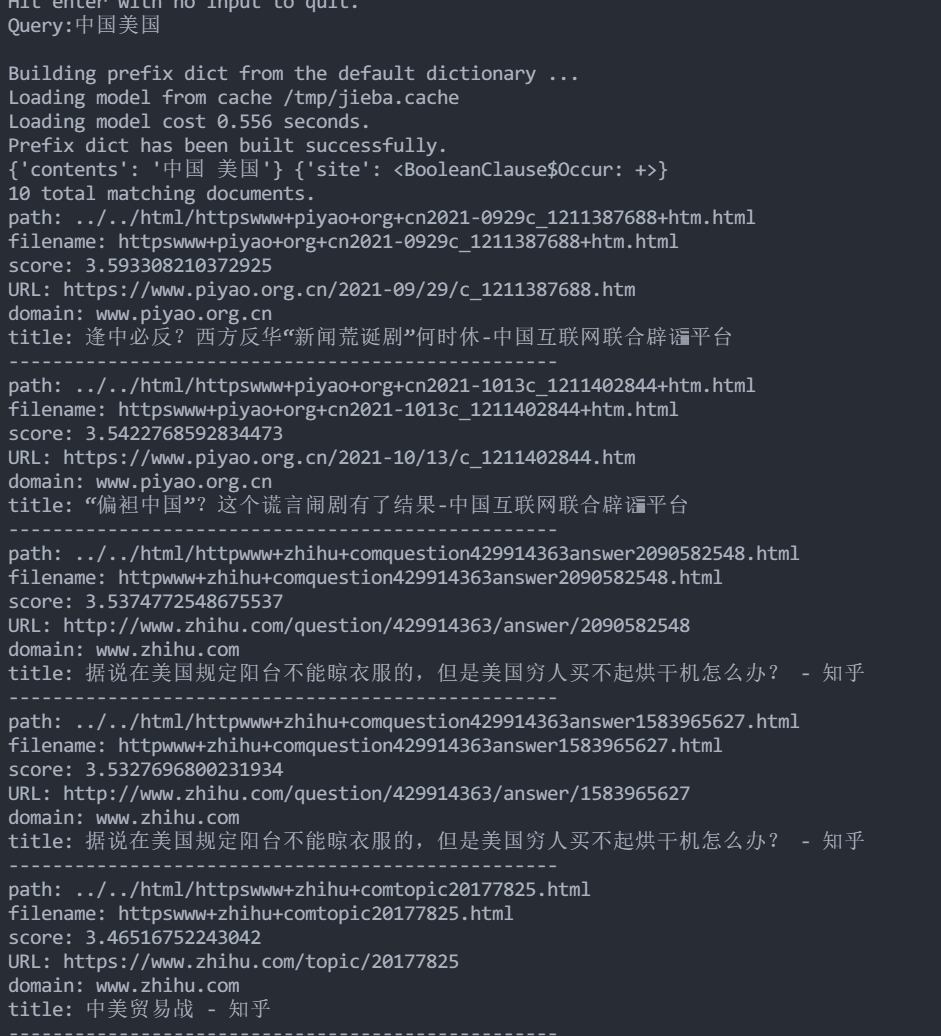
\includegraphics[width=0.6\textwidth]{1_-1.png}
	\centering
	 \caption{默认}
\end{figure}
\begin{figure}[H]
	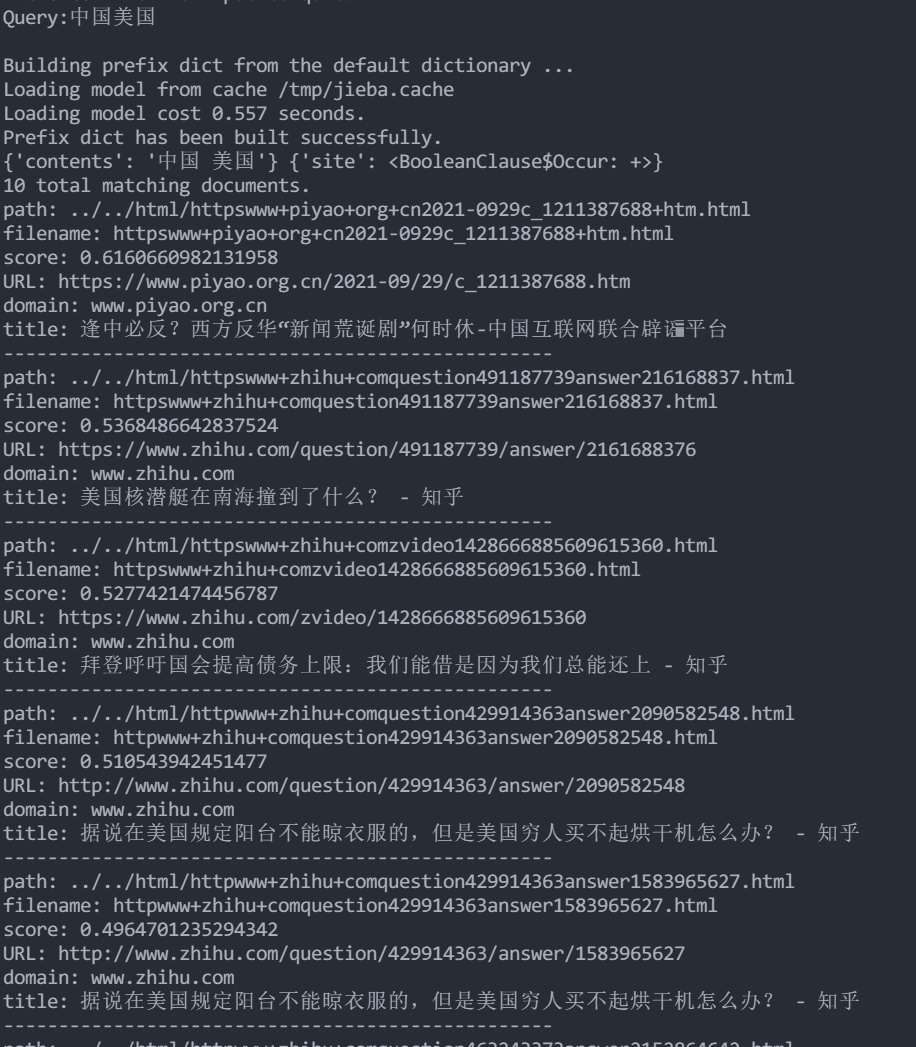
\includegraphics[width=0.6\textwidth]{1_0.png}
	\centering
	 \caption{Similarity0}
\end{figure}
\begin{figure}[H]
	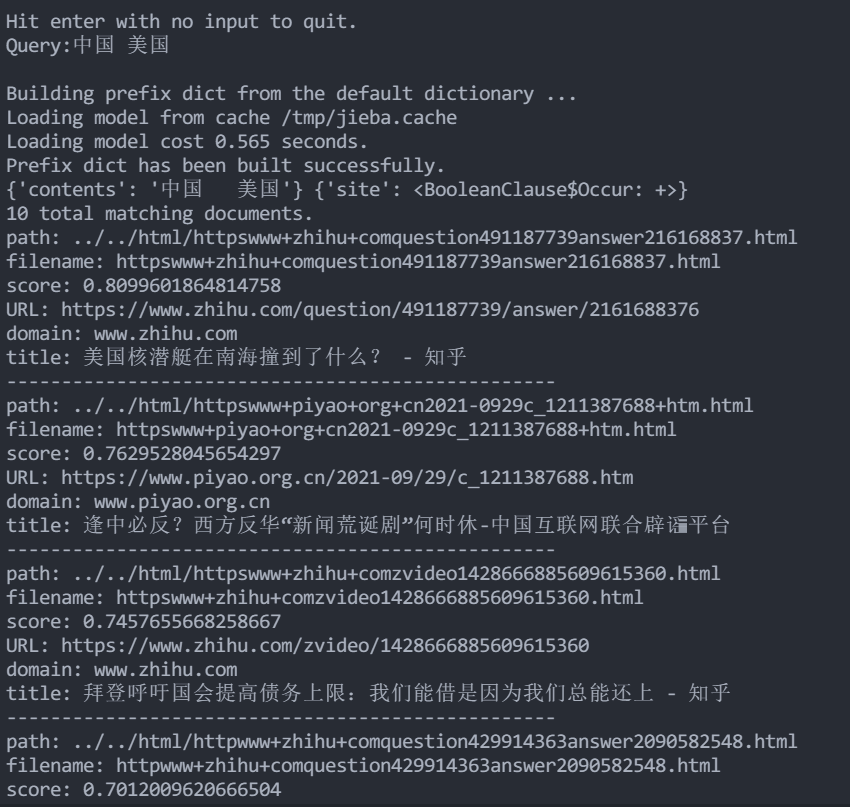
\includegraphics[width=0.6\textwidth]{1_1.png}
	\centering
	 \caption{Similarity1}
\end{figure}

\subsubsection{“最好的编程语言”}

\begin{figure}[H]
	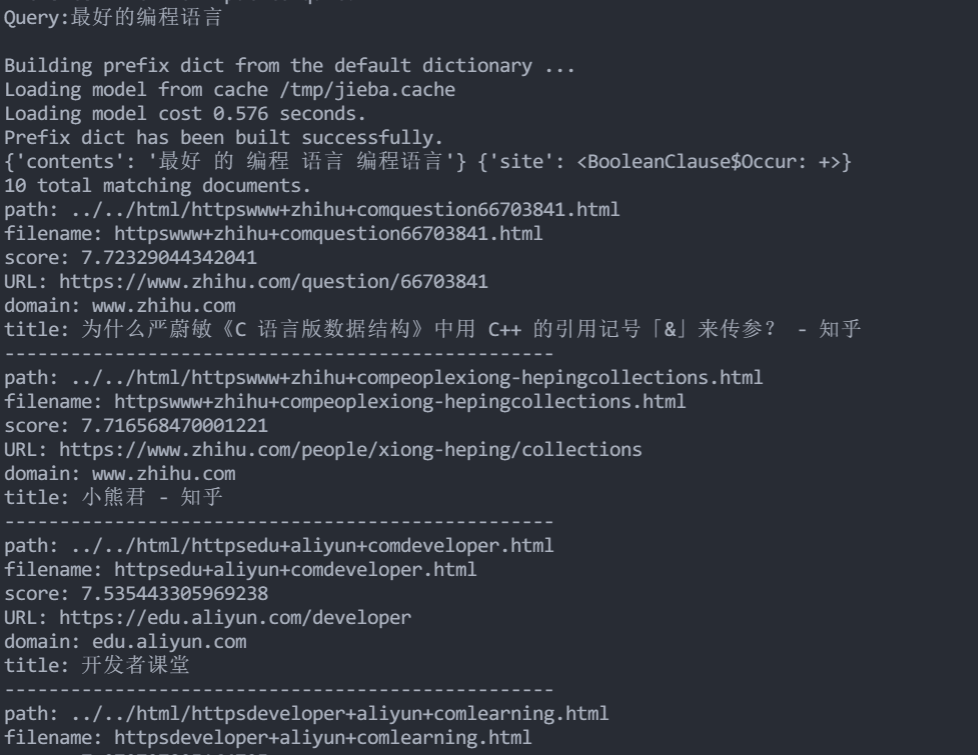
\includegraphics[width=0.6\textwidth]{2_-1.png}
	\centering
	 \caption{默认}
\end{figure}
\begin{figure}[H]
	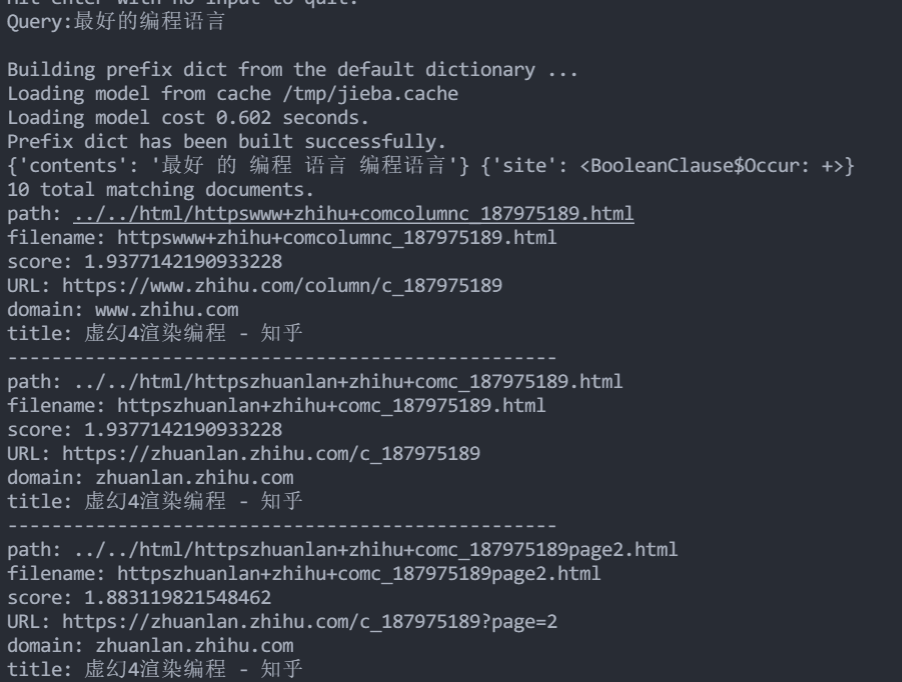
\includegraphics[width=0.6\textwidth]{2_0.png}
	\centering
	 \caption{Similarity0}
\end{figure}
\begin{figure}[H]
	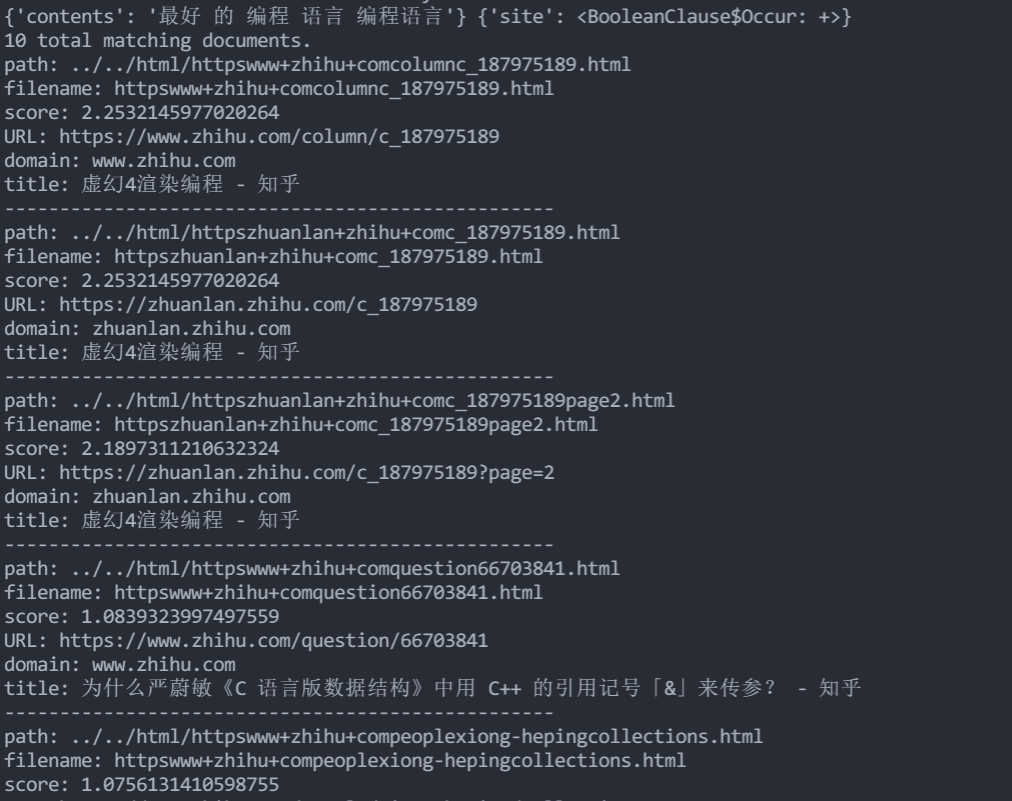
\includegraphics[width=0.6\textwidth]{2_1.png}
	\centering
	 \caption{Similarity1}
\end{figure}

\subsubsection{“中国美食”}

\begin{figure}[H]
	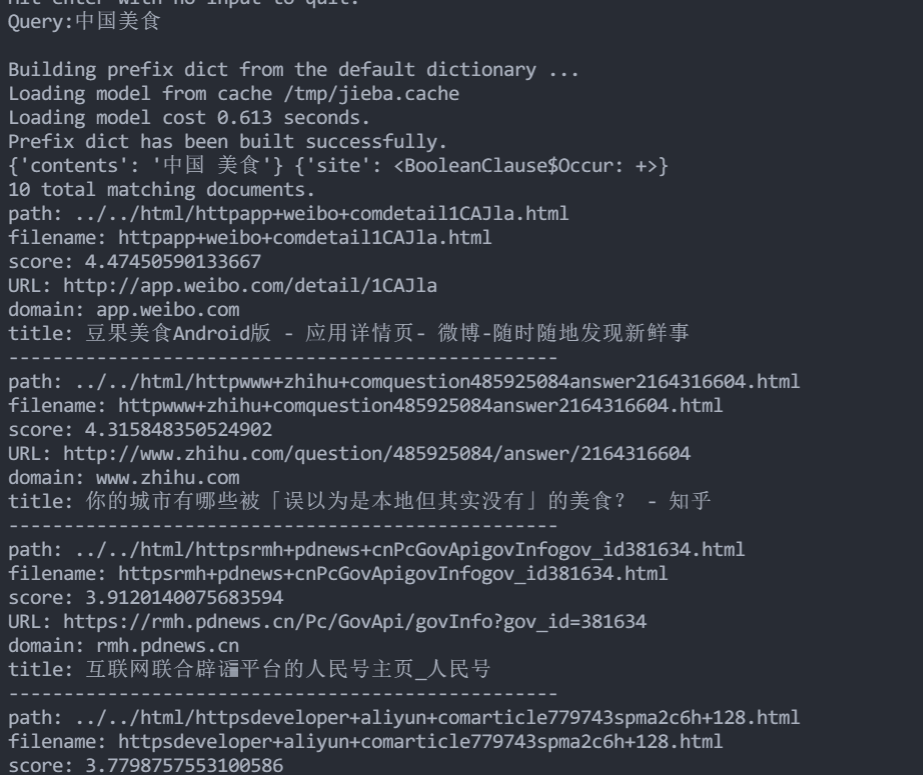
\includegraphics[width=0.6\textwidth]{3_-1.png}
	\centering
	 \caption{默认}
\end{figure}
\begin{figure}[H]
	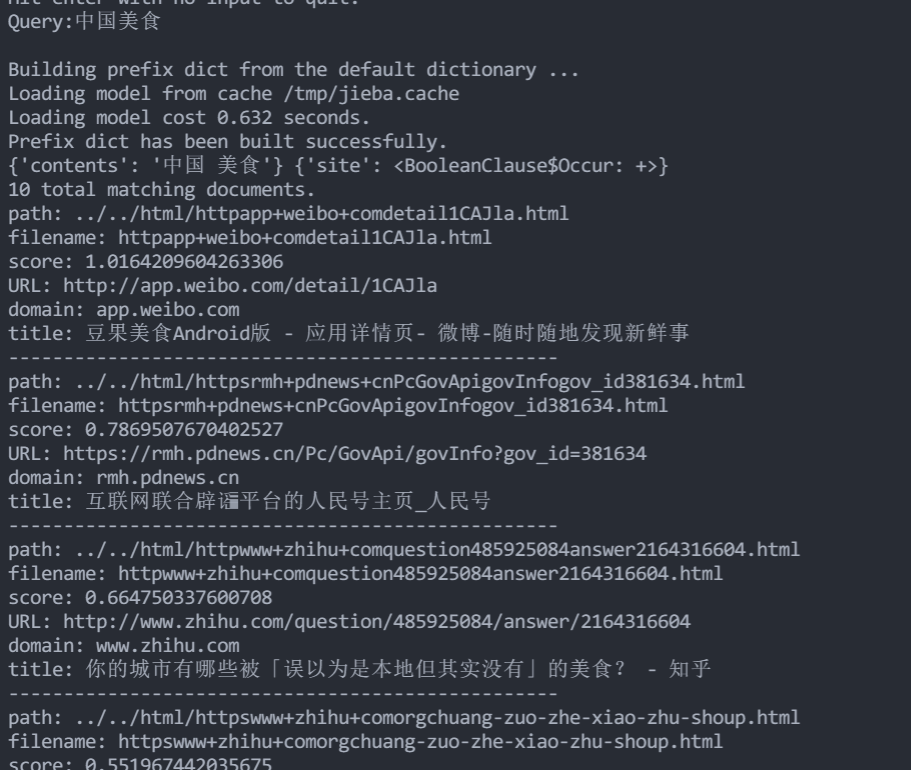
\includegraphics[width=0.6\textwidth]{3_0.png}
	\centering
	 \caption{Similarity0}
\end{figure}
\begin{figure}[H]
	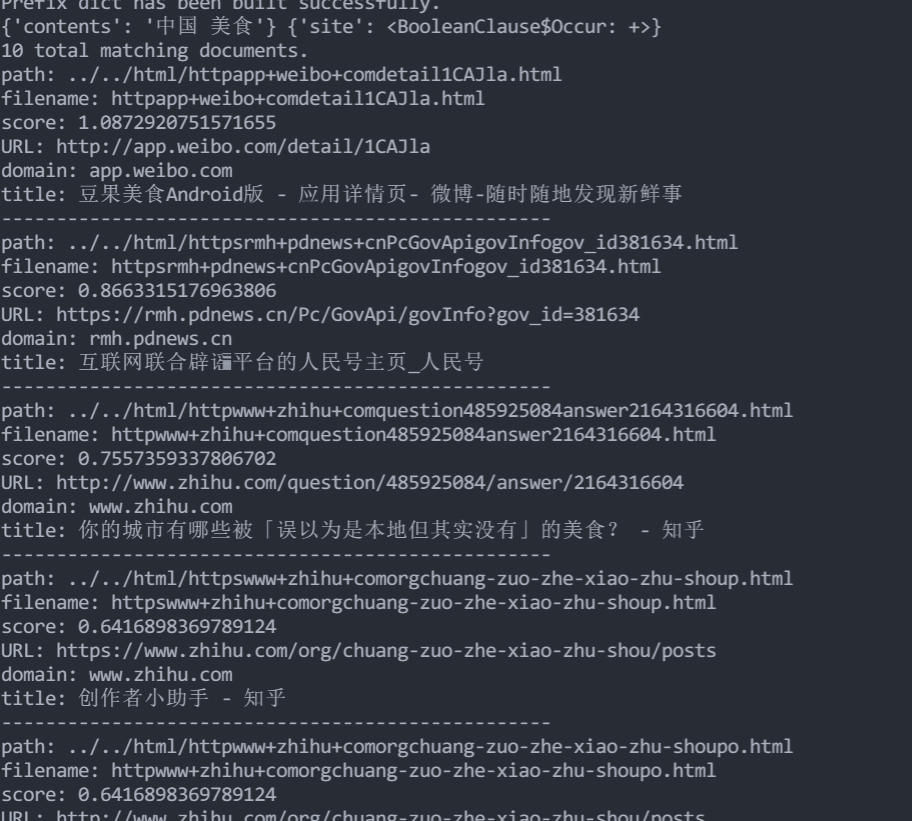
\includegraphics[width=0.6\textwidth]{3_1.png}
	\centering
	 \caption{Similarity1}
\end{figure}

\subsubsection{“搜索引擎”}

\begin{figure}[H]
	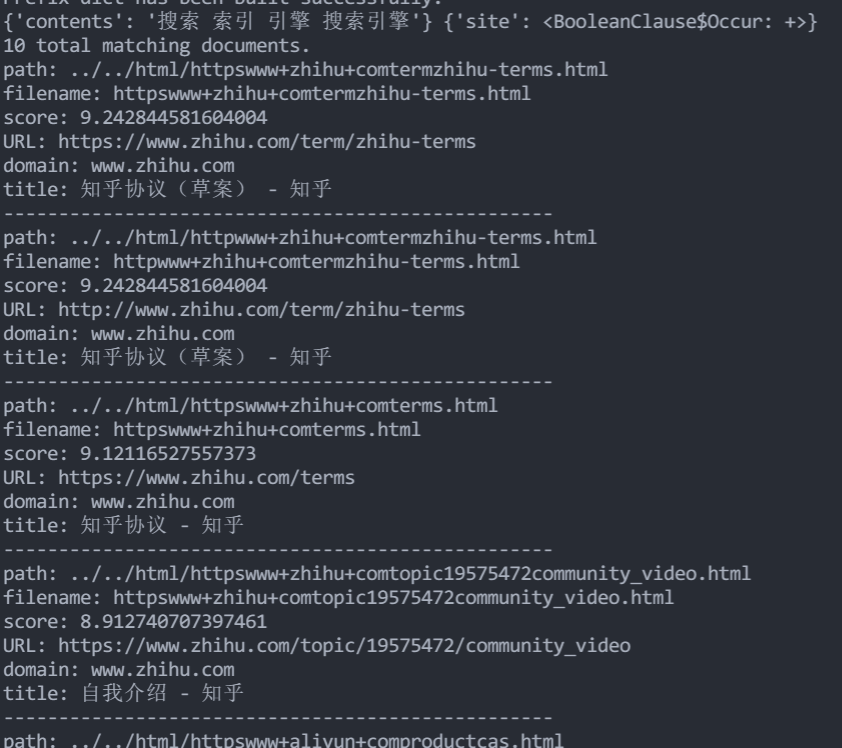
\includegraphics[width=0.6\textwidth]{4_-1.png}
	\centering
	 \caption{默认}
\end{figure}
\begin{figure}[H]
	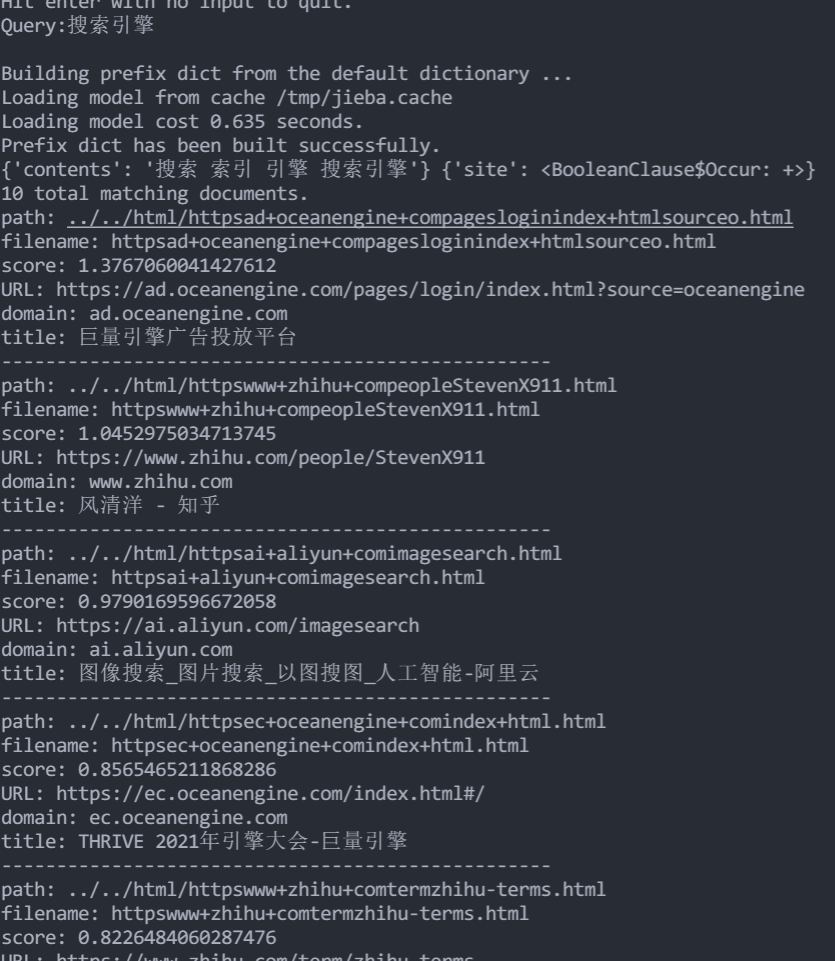
\includegraphics[width=0.6\textwidth]{4_0.png}
	\centering
	 \caption{Similarity0}
\end{figure}
\begin{figure}[H]
	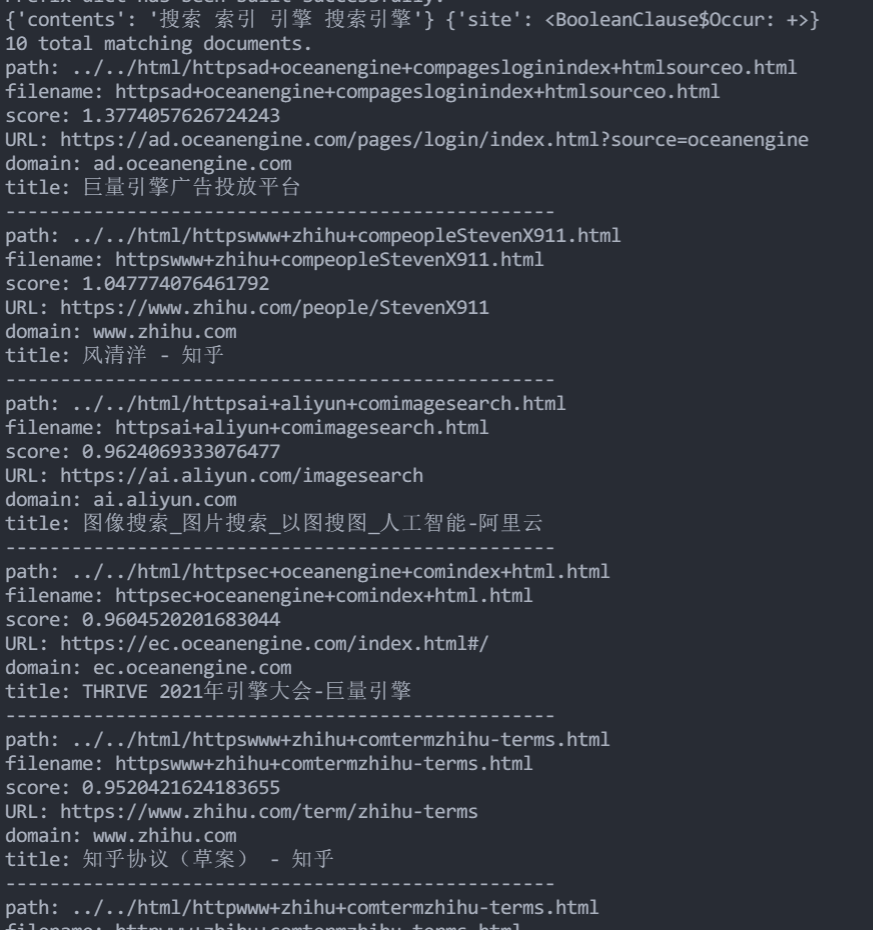
\includegraphics[width=0.6\textwidth]{4_1.png}
	\centering
	 \caption{Similarity1}
\end{figure}

\section{分析与思考}
\begin{itemize}
	\item 从结果来看,用不同函数重写PythonClassicSimilarity对结果影响并不大,但是和Lucene默认方法有一定区别。不同df、idf结果差不多的原因可能是可能是因为测试的网页数目不够大(8000个)或者本身数据对这些变换不敏感。
	\item 观察一些结果可以发现(“搜索引擎”的例子比较明显),重写的tf-idf方法似乎对于keyword出现的次数更敏感,相比之下lucene默认的BM25对全文内容考虑更全面,这二者的优劣有待进一步考量。
\end{itemize}

\end{document}

